% ----------------------------------------------------------------------------
% Copyright (c) 2016 - 2020 by Burkhardt Renz. All rights reserved.
% Die Vorlage für eine Abschlussarbeit in der Informatik am Fachbereich
% MNI der THM ist lizenziert unter einer Creative Commons
% Namensnennung-Nicht kommerziell 4.0 International Lizenz.
%
% Id:$
% ----------------------------------------------------------------------------

\chapter{Frontend Frameworks}

In diesem Kapitel möchte ich zunächst allgemein in die JavaScript-Frontend-Frameworks einführen.
Die Drei aktuell gängigsten Frontend-Frameworks React.js, Angular und Vue.js werden vorgestellt.
\\
\\
An eine moderne Webapplikation werden hohe Anforderungen an den Funktionsumfang durch den Benutzer gestellt.
Die Entwickler einer solchen Webapplikation erwarten eine einheitliche Codequalität und einheitliche Strukturen
für eine bessere Wartbarkeit der Webapplikation.
Um beim Erstellen neuer Webapplikationen den Entwickler dabei zu unterstützen, diese Ziele zu erfüllen,
werden unter anderem entsprechende Frontend Frameworks verwendet.
\begin{quote}
    Front-end frameworks determine the logic, structure, design, behavior,
    and animation of every element you see on-screen when you interact with websites,
    web applications, and mobile apps. \cite{sigdestad22}
\end{quote}
Man kann zwischen UI-Frameworks in HTML und CSS sowie JavaScript-Frameworks unterscheiden.
Letztere dienen als Verbindung zwischen der Darstellung und der Logik im Frontend.
\\
JavaScript-Frameworks beeinflussen den HTML DOM und können HTML sowie CSS Elemente verändern und mit diesen interagieren.
Beim HTML DOM (Document Object Model) handelt es um die hierarchische Anordnung einer HTML-Seite. \cite{whatIsDom}
\\
Aus den Statistiken \ref{fig:stackoverflow_stat} und \ref{fig:google_trends} lässt sich schließen,
dass die drei aktuell gängigsten JavaScript-Frontend-Frameworks React.js, Angular und Vue.js sind.

\begin{figure}[H]
    \centering
    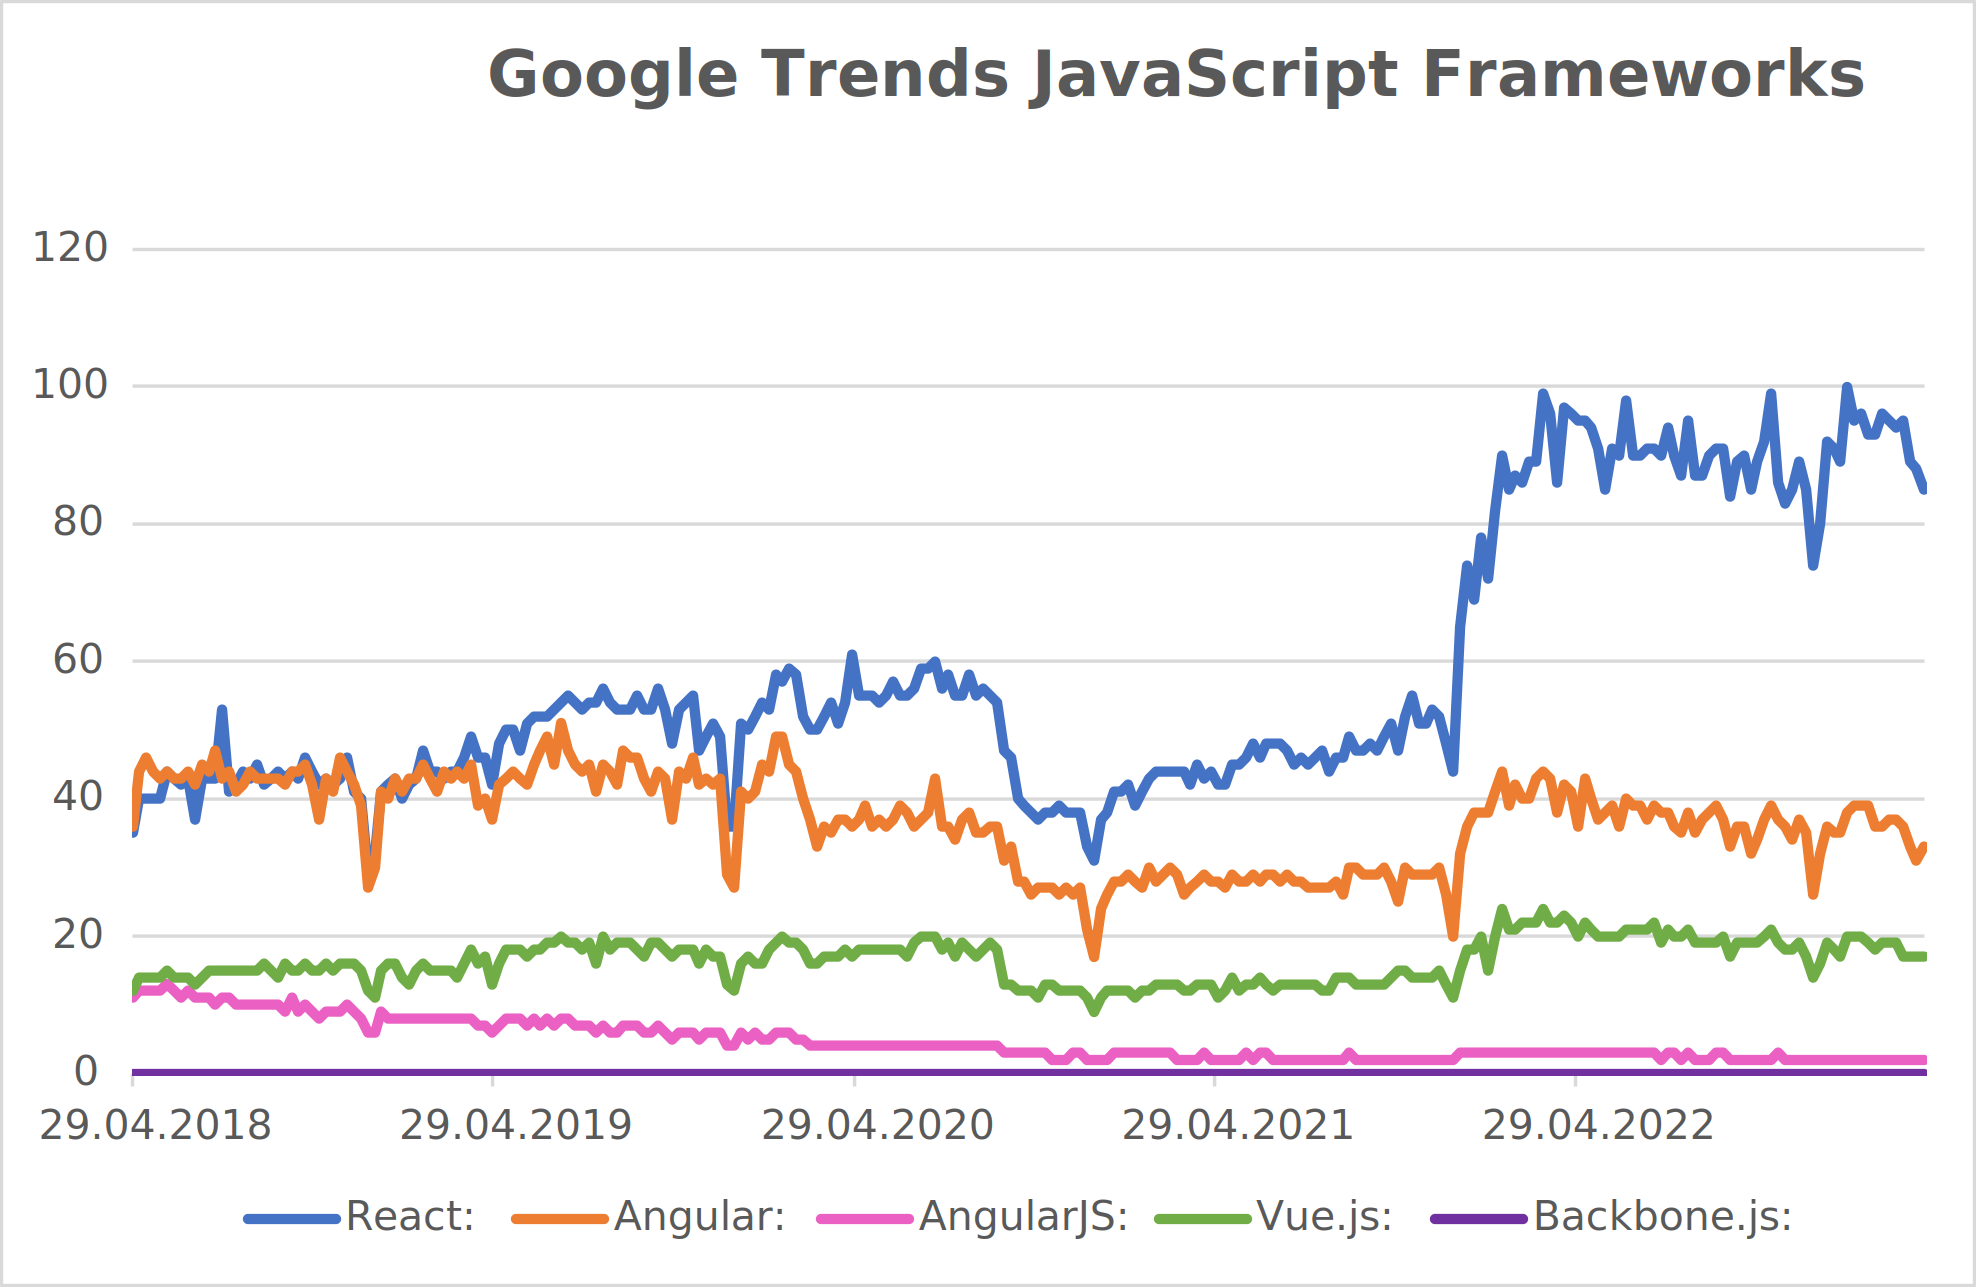
\includegraphics[width=0.6\textwidth]{img/Google Stats/google_frameworks_trends}
    \caption{Google Trends zur Häufigkeit von Suchanfragen nach Frameworks der letzten 5 Jahre \cite{googleTrends}}
    \label{fig:google_trends}
\end{figure}

\begin{figure}[H]
    \centering
    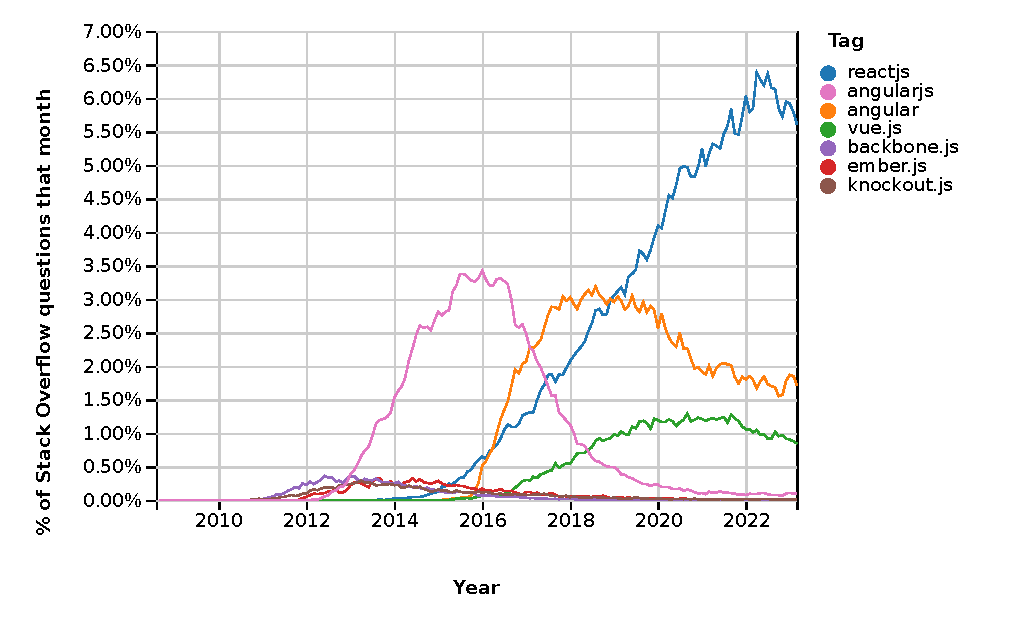
\includegraphics[width=0.8\textwidth]{img/js_frameworks_statistic_stackoverflow}
    \caption{Stack Overflow Statistik zur Häufigkeit von Fragen nach Framework \cite{stackoverflowStats}}
    \label{fig:stackoverflow_stat}
\end{figure}



\section{Vue.js}
Vue.js wurde von Evan You als Nebenprojekt entwickelt und erschien 2014.
Das Projekt finanziert sich laut eigenen Angaben aus Spenden und
wird von sowohl Vollzeitentwicklern und Freiwilligen gepflegt \cite{vueFAQ}.
Nach Google Trends und Stack Overflow Statistik ist es aktuell das drittbeliebteste
Frontend Framework \cite{googleTrends} \cite{stackoverflowStats}.
Hohe Beliebtheit hat das Framework in China (siehe Abb.\ref{fig:google_trends_world}).
Besonderheit des Frameworks ist, dass es in seiner Grundform keine 20 KB groß ist \cite[S. 523]{bin2019}.

\section{Angular}
Angular wurde von Google entwickelt und erschien 2016 ursprünglich als \emph{AngularJs 2.0},
dabei handelt sich um eine vollständige Neuimplementierung in TypeScript unabhängig der Codebasis des Vorgängers AngularJS.
Die Pflege und Weiterentwicklung wird vom Angular Team von Google durchgeführt \cite[S. 209-210]{bin2019}.
Nach Google Trends und Stack Overflow Statistik ist es aktuell das zweitbeliebteste
Frontend Framework \cite{googleTrends} \cite{stackoverflowStats}.

\section{React.js}
Das laut Stack Overflow Statistik und Google Trends gefragteste Frontend Framework ist aktuell React.js \cite{googleTrends} \cite{stackoverflowStats}.
React.js wurde von Facebook entwickelt und 2013 veröffentlicht.
Das Ziel bestand darin, ein Framework zu entwickeln,
das den Anforderungen an Skalierbarkeit und Wartbarkeit gerecht wird,
wie sie für eine umfangreiche Webapplikation wie Facebook erforderlich sind \cite[S. 1]{gackenheimer2015introduction}.
Mittlerweile ist es ein Open-Source-Projekt des Facebookmutterkonzerns Meta.
React setzt dabei auf \emph{JavaScript syntax extension} (JSX), was einen hybriden Code aus JavaScript und HTML-Elementen ermöglicht. \cite{react}


\begin{figure}[!htb]
    \centering
    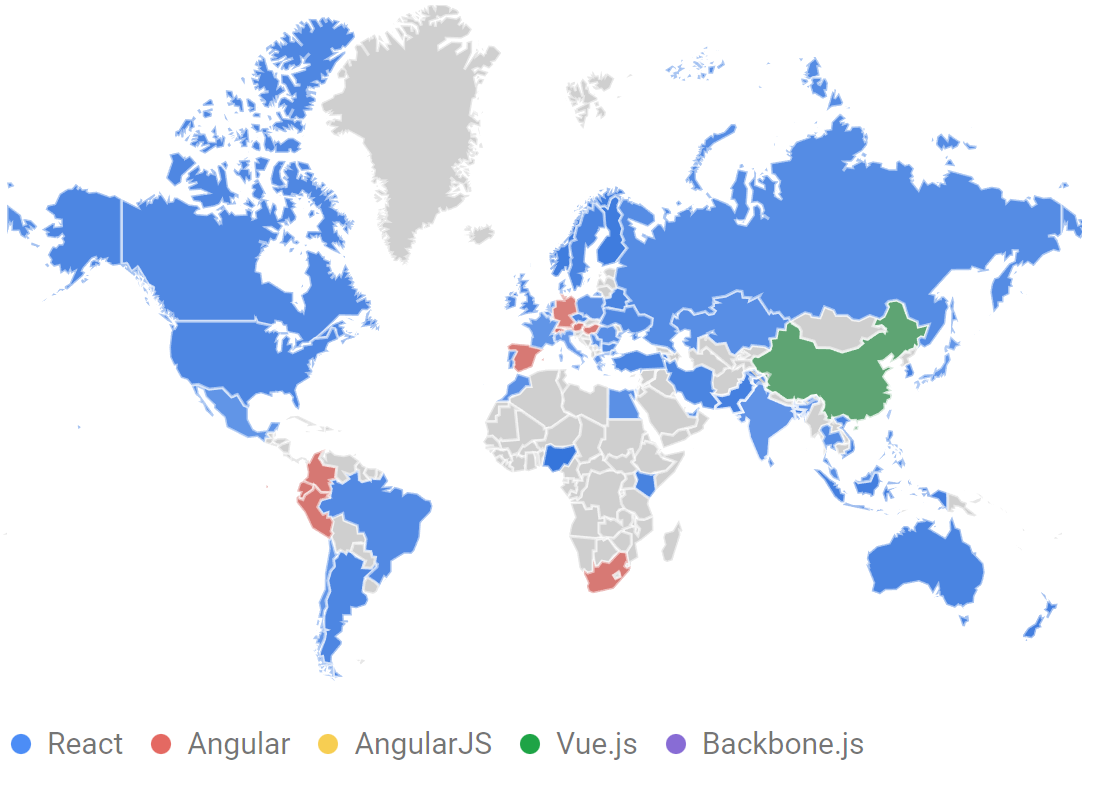
\includegraphics[width=0.6\textwidth]{img/Google Stats/2023-04-26 12_20_26-React, Angular, AngularJS, Vue.js, Backbone.js - Erkunden - Google Trends}
    \caption{Googlge Trends Weltweiteverteilung von Suchanfragen nach Frameworks der letzten 5 Jahre \cite{googleTrends}}
    \label{fig:google_trends_world}
\end{figure}
% ----------------------------------------------------------------------------
